% Options for packages loaded elsewhere
\PassOptionsToPackage{unicode}{hyperref}
\PassOptionsToPackage{hyphens}{url}
\PassOptionsToPackage{dvipsnames,svgnames,x11names}{xcolor}
%
\documentclass[
  11pt,
]{article}
\usepackage{amsmath,amssymb}
\usepackage{iftex}
\ifPDFTeX
  \usepackage[T1]{fontenc}
  \usepackage[utf8]{inputenc}
  \usepackage{textcomp} % provide euro and other symbols
\else % if luatex or xetex
  \usepackage{unicode-math} % this also loads fontspec
  \defaultfontfeatures{Scale=MatchLowercase}
  \defaultfontfeatures[\rmfamily]{Ligatures=TeX,Scale=1}
\fi
\usepackage{lmodern}
\ifPDFTeX\else
  % xetex/luatex font selection
\fi
% Use upquote if available, for straight quotes in verbatim environments
\IfFileExists{upquote.sty}{\usepackage{upquote}}{}
\IfFileExists{microtype.sty}{% use microtype if available
  \usepackage[]{microtype}
  \UseMicrotypeSet[protrusion]{basicmath} % disable protrusion for tt fonts
}{}
\makeatletter
\@ifundefined{KOMAClassName}{% if non-KOMA class
  \IfFileExists{parskip.sty}{%
    \usepackage{parskip}
  }{% else
    \setlength{\parindent}{0pt}
    \setlength{\parskip}{6pt plus 2pt minus 1pt}}
}{% if KOMA class
  \KOMAoptions{parskip=half}}
\makeatother
\usepackage{xcolor}
\usepackage[margin=1in]{geometry}
\usepackage{longtable,booktabs,array}
\usepackage{calc} % for calculating minipage widths
% Correct order of tables after \paragraph or \subparagraph
\usepackage{etoolbox}
\makeatletter
\patchcmd\longtable{\par}{\if@noskipsec\mbox{}\fi\par}{}{}
\makeatother
% Allow footnotes in longtable head/foot
\IfFileExists{footnotehyper.sty}{\usepackage{footnotehyper}}{\usepackage{footnote}}
\makesavenoteenv{longtable}
\usepackage{graphicx}
\makeatletter
\def\maxwidth{\ifdim\Gin@nat@width>\linewidth\linewidth\else\Gin@nat@width\fi}
\def\maxheight{\ifdim\Gin@nat@height>\textheight\textheight\else\Gin@nat@height\fi}
\makeatother
% Scale images if necessary, so that they will not overflow the page
% margins by default, and it is still possible to overwrite the defaults
% using explicit options in \includegraphics[width, height, ...]{}
\setkeys{Gin}{width=\maxwidth,height=\maxheight,keepaspectratio}
% Set default figure placement to htbp
\makeatletter
\def\fps@figure{htbp}
\makeatother
\setlength{\emergencystretch}{3em} % prevent overfull lines
\providecommand{\tightlist}{%
  \setlength{\itemsep}{0pt}\setlength{\parskip}{0pt}}
\setcounter{secnumdepth}{-\maxdimen} % remove section numbering
\usepackage{amsmath,amssymb}
\usepackage{xurl}
\ifLuaTeX
  \usepackage{selnolig}  % disable illegal ligatures
\fi
\IfFileExists{bookmark.sty}{\usepackage{bookmark}}{\usepackage{hyperref}}
\IfFileExists{xurl.sty}{\usepackage{xurl}}{} % add URL line breaks if available
\urlstyle{same}
\hypersetup{
  pdftitle={When Control Corrupts Information},
  pdfauthor={Dr.~Jan-Hendrik Weinert},
  colorlinks=true,
  linkcolor={Maroon},
  filecolor={Maroon},
  citecolor={Blue},
  urlcolor={Blue},
  pdfcreator={LaTeX via pandoc}}

\title{When Control Corrupts Information}
\usepackage{etoolbox}
\makeatletter
\providecommand{\subtitle}[1]{% add subtitle to \maketitle
  \apptocmd{\@title}{\par {\large #1 \par}}{}{}
}
\makeatother
\subtitle{Feasible Auditing, Report Use, and the Nonmonotone Demand for
Protection}
\author{Dr. Jan-Hendrik Weinert}
\date{19 October 2026}


% Publication formatting edition, 19 October 2026. Scientific equations unchanged.
\usepackage{xurl,needspace,etoolbox}
\geometry{a4paper,margin=25.4mm}
\hypersetup{hidelinks,pdfauthor={Dr. Jan-Hendrik Weinert}}
\setlength{\parindent}{1.2em}
\setlength{\parskip}{3pt plus 1pt}
\setlength{\emergencystretch}{3em}
\hfuzz=0.2pt
\raggedbottom
\pagestyle{plain}
\makeatletter
\renewcommand{\@seccntformat}[1]{\csname the#1\endcsname\ifstrequal{#1}{section}{.}{}\quad}
\renewcommand{\maketitle}{%
  \begin{center}
  {\LARGE\bfseries\@title\par}
  \vspace{0.8em}
  {\normalsize\@author\par}
  \vspace{0.35em}
  {\small\@date\par}
  \end{center}
  \vspace{0.4em}}
\renewenvironment{abstract}{%
  \begin{center}\small\bfseries Abstract\end{center}
  \begin{list}{}{\setlength{\leftmargin}{0.5in}\setlength{\rightmargin}{0.5in}}
  \item[]\small\setlength{\parindent}{0pt}\ignorespaces
}{\end{list}\vspace{0.6em}}
\makeatother

\begin{document}
\maketitle
\begin{abstract}
How should organizations combine independent audits with the use of employee reports for evaluation? We solve a finite-menu governance problem in which workers separately prevent defects, discover them and disclose findings. Audits verify occurrences but cannot prove prior awareness, excluding concealment penalties from the implementable benchmark. At fixed incidence, audits have no direct discovery or disclosure effect. Jointly optimizing audit intensity and report use yields a globally certified nonmonotone protection policy: higher information value can reduce, then increase, report use before full protection becomes optimal. Total optimized information remains monotone in its value. Complete proofs, boundary cases and synthetic interval certificates establish the result within the constrained menu; no empirical discovery or dishonesty effect is identified.
\end{abstract}
\section{1. Introduction}\label{the-governance-question}

Operational records are both inputs to learning and evidence used to
evaluate the people who produce them. An organization choosing a
reporting policy must consider prevention, discovery, disclosure, the
independent information produced by audits, and the resource cost of
protecting a learning channel. A higher report count is not
automatically better information, and a lower count is not automatically
lower operational risk.

This paper studies a restricted but implementable policy-design problem.
The organization chooses an audit intensity and a report-linked
evaluation charge from a finite menu. A contractual liability cap rules
out some combinations. Audits can establish a defect and sometimes its
diagnostic context; they cannot establish whether an employee previously
knew about it. No penalty is imposed merely by labeling an omitted
report deliberate concealment. Individual report use can still
discourage disclosure, because a submitted report is observable.
Protection means reducing this report-linked charge, not abolishing
independent accountability.

The principal result is a nonmonotone optimal demand for protection.
When learning becomes more valuable, choosing a stronger audit
technology can make increased individual report use optimal even though
it reduces worker reporting sensitivity. Independent diagnostic
information replaces some worker-produced information; saved protection
costs and prevention gains can justify that substitution. This is not
the claim that controls generally improve information or that
concealment penalties are desirable. It occurs in the feasible benchmark
with no awareness-contingent penalty.

The article supplies an exact finite-menu solution and parameter
regions, rather than a comparison of two selected regimes. Finite menus
represent administratively approved audit and access-control packages.
Optimality is relative to that menu, a fixed occurrence penalty, and a
fixed reporting reward. It is not optimality over all contracts. The
upper-envelope method itself is elementary. The substantive result is a
counterexample to monotone protection, obtained with endogenous
prevention, discovery, disclosure, combined audit/report information,
and enforceability constraints. Its importance outside this model
remains an empirical question.

\section{2. The predecessor and the contribution
boundary}\label{the-predecessor-and-the-contribution-boundary}

The actual author-hosted published article by Graff Zivin and Pfaff
(2004), not a working version, is the closest predecessor. Its results
are equation-based rather than numbered propositions:

\begin{longtable}[]{@{}
  >{\raggedright\arraybackslash}p{(\columnwidth - 2\tabcolsep) * \real{0.5000}}
  >{\raggedright\arraybackslash}p{(\columnwidth - 2\tabcolsep) * \real{0.5000}}@{}}
\toprule\noalign{}
\begin{minipage}[b]{\linewidth}\raggedright
Published location
\end{minipage} & \begin{minipage}[b]{\linewidth}\raggedright
Existing implication
\end{minipage} \\
\midrule\noalign{}
\endhead
\bottomrule\noalign{}
\endlastfoot
Section 2.2, equations (4)-(5), pp.~941-942 & Reporting increases
exposure and distorts adoption despite incentives for correction. \\
Section 3.1, equations (6)-(8), pp.~942-943 & Differentiated penalties
can equate expected exposure and restore adoption incentives. \\
Section 3.2, equations (9)-(12), pp.~943-945 & Hidden physician
detection/reporting effort and agency costs already enter. \\
Section 4.1, pp.~946-947; Appendix A, pp.~947-948 & Observable proxies
and outcome-contingent incentives address unobserved effort. \\
\end{longtable}

Thus sanctions deterring reports, endogenous detection, and the general
incentive-design problem are not new. Here the added object is joint
menu choice under a liability cap, with audit-produced diagnostic
signals and no inference of awareness. The nonmonotonicity result is not
implied by the predecessor's stated policy equalization conditions.

The broader boundary is also important. Pfaff and Sanchirico (2000)
already analyze self-investigation and correction incentives, including
observability problems. Kaplow and Shavell (1994) characterize optimal
self-reporting enforcement, including enforcement-resource benefits. A
paper cannot claim originality merely by adding audit costs or calling
report-use restrictions governance. Their primary publisher or author
records were verified; those records support the broad comparison, not a
claim to have exhausted every theorem in their restricted full texts.

Dai (2026), a particularly close recent comparison, jointly optimizes
regulatory audit intensity and penalties under limited liability. Its
Lemmas 1-2 concern self-audit timing; Proposition 1 characterizes
regulatory policies. The present article therefore does not claim joint
audit/penalty design or audit crowd-out as new. Its distinct target is
how the value of diagnostic learning changes optimal report-use
protection when worker discovery and disclosure are separate.

Wang, de Véricourt, and Sun (2024) solve a richer dynamic
audit/remediation problem with evasion; the consulted author
manuscript's Theorem 1 establishes optimal prompt disclosure in its
contract space. That result reinforces why our restricted-menu
optimality cannot be advertised as a general optimal-contract theorem.
Strausz (2006), compared using the October 2004 manuscript and verified
final metadata, connects reporting, audit precision, and rents. Here
audit source independence and costly suppression are different
assumptions, not discoveries that reporting and auditing interact.

Bénabou and Tirole (2016) place multitasking within competitive
screening. The verified final publication is distinct from the March
2013 author manuscript consulted for its framework. Edmondson (1996) and
Bernstein (2012) supply direct organizational precedents on detection,
learning, visibility, and concealment. Maas and van Rinsum (2013)
caution that identification can sometimes improve reporting honesty.
These precedents motivate allowing both information losses and benefits
from accountability. The proposed contribution is narrower than
discovering endogenous organizational information.

\section{3. Worker behavior and enforceable
policies}\label{worker-behavior-and-enforceable-policies}

\subsection{3.1 Production of defects and
reports}\label{production-of-defects-and-reports}

One worker handles one item. Preventive effort \(e\geq0\) costs
\(c_e e^2/2\) and makes a defect occur with probability

\[p(e)=p_0e^{-e},\qquad 0<p_0<1.\]

Investigative attention \(d\in[0,1]\) costs \(kd^2/2\), whether or not a
defect exists, and discovers a true defect with probability \(d\).
Following discovery, the worker chooses concealment intensity
\(c\in[0,1]\), at real expected cost \(\eta c^2/2\) per discovery.
Disclosure then occurs with probability \(1-c\). This reduced-form
convex concealment technology represents the cost of suppressing
discovered information; it is not a statement about observed employee
intent. Reporting sensitivity and raw report probability are

\[q=d(1-c),\qquad r=pq. \tag{1}\]

There are no false positives in the behavioral baseline. Their empirical
measurement is addressed separately. A discovery yields private
immediate remediation benefit \(u\geq0\) even without disclosure. A
disclosed finding earns a reward \(v\geq0\) and incurs report-use
evaluation charge \(s\geq0\). A randomly selected independent audit,
with probability \(a\), imposes occurrence penalty \(b\geq0\) if a
defect exists, whether or not it was reported. Let \(h>0\) be private
defect harm and \(H=h+ab\).

Audits occur after the worker reporting window and immediate private
remediation. They do not substitute for the immediate benefit \(u\).
This timing/separability assumption is important: awareness-blind audits
can directly crowd out investigation in other models, including
audit-substitution settings such as Dai (2026). Theorem 2 below is a
benchmark within (2), not an impossibility theorem across all feasible
technologies.

An awareness-contingent penalty would be \(F\) per discovered but
concealed defect caught by an audit. The general utility expression is

\[U=-\frac{c_e e^2}{2}-Hp+
 pd\left[u+(v-s)(1-c)-\frac{\eta c^2}{2}-aFc\right]-\frac{kd^2}{2}. \tag{2}\]

The governance analysis imposes \textbf{\(F=0\)}. Occurrence alone does
not prove awareness. A report-use charge is enforceable because
submission itself is observable; an occurrence penalty relies on the
independent artifact. Charges are assumed contractual monetary
transfers, not uncontrolled reputational or career damage. Fixed
compensation satisfies participation. This assumption permits a coherent
inclusive-surplus objective and restricts its organizational
interpretation.

\subsection{3.2 Feasible menu and
liability}\label{feasible-menu-and-liability}

The organization commits before worker choices to a deterministic pair
\((a,s)\) in a finite candidate set \(\mathcal A\times\mathcal S\).
Auditing capacity bounds \(a\leq\bar a\leq1\). A gross per-item
liability cap \(B\) requires

\[s+b\mathbf1\{a>0\}\leq B. \tag{3}\]

If an audit can occur, an audited and reported defect can incur both
charges; if \(a=0\), only the report charge can occur. Equation (3) caps
gross negative transfers before the separate reporting reward. It is a
contractual cap, not an estimate of a jurisdiction's liability law. No
policy may charge an unobserved awareness fine. Audit probability is
selected before seeing reports and is not targeted by their contents.

Real audit cost is \(K(a)=\kappa a^2/2\), \(\kappa>0\). Reduced report
use requires access restrictions and enforcement of a use boundary, with
real channel cost \(C(s)=\gamma\phi(s)\), \(\gamma>0\), where

\[\phi(s)=\left[\max\{1-s/\bar s,0\}\right]^2. \tag{4}\]

Full protection is \(s=0\), not zero audit intensity. The specified cost
schedule is an assumption about implementing protection. It is not a
finding that every organization faces quadratic governance costs. The
menu, cap, capacity, and cost schedule together define the constrained
design problem. Random policy mixing is unnecessary for a linear
objective over independently treated items: an average of deterministic
policy surpluses cannot exceed their maximum. Hidden lotteries that
workers cannot observe before choosing actions would be a different
contract space.

\subsection{3.3 A global worker solution, including zero
information}\label{a-global-worker-solution-including-zero-information}

Write \([x]_0^1=\max\{0,\min\{1,x\}\}\) and \(g_+=\max\{g,0\}\). For a
continuation following discovery,

\[c^*=\left[\frac{s-v-aF}{\eta}\right]_0^1,\qquad
 g=u+(v-s)(1-c^*)-\frac{\eta(c^*)^2}{2}-aFc^*. \tag{5}\]

For all policies under consideration assume a common bound \(G\geq g_+\)
satisfying

\[\frac{p_0G}{k}<1,\qquad h>\frac{2p_0G^2}{k}. \tag{6}\]

These primitive bounds deliberately exclude saturated attention along
the effort domain; they do not exclude zero attention or either
concealment boundary. For nonnegative \(s,F\), one may take \(G=u+v\). A
tighter policy-specific bound can also be used.

\textbf{Theorem 1 (global response).} Under (6), each policy has a
unique preventive effort and investigative attention:

\[d^*=pg_+/k,\qquad
 c_e e=pH-p^2g_+^2/k. \tag{7}\]

The effort equation has exactly one positive solution on \([0,\infty)\).
When \(g\leq0\), attention and reporting are zero. The continuation
value \(c^*\) is still well defined, but no realized concealment rate is
observed if nothing is discovered. When \(s\leq v+aF\), concealment is
zero; when \(s\geq v+aF+\eta\), disclosure is zero. Equations (5)-(7)
remain valid at all these boundaries and are continuous in policy. All
proofs appear in Appendix A.

\section{4. What implementable audits do and do not
do}\label{what-implementable-audits-do-and-do-not-do}

\subsection{4.1 The feasible benchmark: no direct attention
reversal}\label{the-feasible-benchmark-no-direct-attention-reversal}

With \(F=0\), \(c\) and \(g\) depend on \(s\) but not on \(a\). Let

\[\Delta=c_e+Hp-2p^2g_+^2/k>0.\]

\textbf{Theorem 2 (awareness-blind audit benchmark).} At fixed defect
incidence \(p\), changing \(a\) leaves discovery and disclosure
unchanged, including zero attention and concealment boundaries. With
endogenous prevention,

\[e_a=pb/\Delta,\qquad p_a=-pe_a,\qquad q_a=-e_aq. \tag{8}\]

Thus audit-induced reductions in reporting sensitivity in this benchmark
are entirely mediated by prevention. There is no fixed-incidence audit
corruption effect. If \(b=0\) or \(q=0\), the corresponding derivative
is zero. One cannot reinterpret (8) as evidence that employees hide
known findings when auditing increases.

At fixed \(a\), greater report-linked charge \(s\) can increase
prevention and reduce discovery and disclosure. In an interior
concealment region with \(g>0\),

\[e_s=2pd(1-c)/\Delta,\qquad
 q_s=-e_sq-p(1-c)^2/k-d/\eta. \tag{9}\]

The second term is the direct discovery loss; the third is disclosure
conditional on discovery; the first is the indirect prevention margin.
At concealment corners the derivative of \(c\) is zero locally; at
\(g\leq0\), reporting is zero. These effects do not establish that full
protection maximizes welfare.

\subsection{4.2 Information from both
sources}\label{information-from-both-sources}

Each item has a latent binary root-cause label \(\theta\) with prior one
half, independent of whether a defect occurs. A worker report reveals
the label. An audit always verifies occurrence and, independently of
worker reporting conditional on a defect, recovers the label with
probability \(\rho\in[0,1]\). Audit diagnostic capability is not proof
of the worker's prior awareness. An audit can reconstruct a cause
without reconstructing an employee's knowledge history.

Counting each defect at most once, total occurrence-detection
probability and diagnostic-label arrival probability per item are
respectively

\[T=p[q+a(1-q)],\qquad
 I=p[q+a\rho(1-q)]. \tag{10}\]

Conditional diagnostic sensitivity is \(J=I/p\). Reports and audits can
overlap; adding \(pq+pa\rho\) without subtracting overlap would
overstate information. When \(\rho=1\), \(I=T\); when \(\rho=0\),
auditing still verifies occurrences, but diagnostic learning in this
specification comes from worker reports only.

A subsequent remedy decision pays \(V\) if its chosen binary action
matches \(\theta\) and zero otherwise. With no label, optimal expected
payoff is \(V/2\); with a label, it is \(V\). Since the absence of a
label is independent of \(\theta\), incremental decision value is
\(LI\), where \(L=V/2\). Any separate value assigned to occurrence
verification can be added as \(MT\), \(M\geq0\). We set \(M=0\) for the
explicit example, rather than counting occurrence information as
worthless in every application. The general finite-menu solution below
allows \(M\geq0\).

Under Theorem 2, combined conditional diagnostic sensitivity and
unconditional learning supply obey

\[J_a=\rho(1-q)-(1-a\rho)e_aq,\]

\[I_a=p\{\rho(1-q)-e_a[a\rho+2(1-a\rho)q]\}. \tag{11}\]

At fixed incidence, \(J_a=\rho(1-q)\geq0\). With prevention, either sign
of (11) is possible. A decrease in learning opportunities because fewer
defects occur is not direct corruption of discovery or disclosure. The
design problem must value real prevention separately from the supply of
diagnostic signals.

\subsection{4.3 Exact boundary of the earlier perverse-audit
mechanism}\label{exact-boundary-of-the-earlier-perverse-audit-mechanism}

For comparison only, suppose an external technology could prove
awareness, so \(F>0\) were feasible. This technology is not assumed
available or optimized here. At fixed \(p\), allow the general attention
cap \(d=[pg/k]_0^1\), even outside (6).

\textbf{Theorem 3 (primitive reversal region).} Put \(x=s-v\) and
\(t=(u-x)/\eta\). A strictly negative fixed-incidence derivative
\(\partial q/\partial a\) is possible only with \(0<c<1\) and
\(0<pg/k<1\). In this region,

\[g=u-x+\eta c^2/2,\qquad
 \left.\frac{\partial q}{\partial a}\right|_p
 =\frac{pF}{k}\left[t+\frac32c^2-c\right]. \tag{12}\]

It is negative exactly where \(g>0\) and

\[c_-<c<c_+,\quad
 c_\pm=\frac{1\pm\sqrt{1-6t}}{3}, \tag{13}\]

intersected with \(0<c<1\) and reachable \(c=(x-aF)/\eta\). Real
distinct roots require \(t<1/6\). In particular, \(u-x\geq\eta/6\) rules
out reversal globally. In a saturated-attention region the derivative is
\(F/\eta>0\); in the interiors of zero attention, zero concealment, or
full concealment it is zero. At kinks the function is continuous and
one-sided derivatives follow the adjacent formulas. Setting \(F=0\)
removes the entire fixed-incidence reversal, not just its numerical
example.

This result delimits a specific penalty technology. It does not
recommend implementing awareness fines or claiming that an omitted
report proves awareness. For example, at \(p=.1\), \(u=.6\), \(s=.7\),
\(v=.1\), \(a=.2\), \(F=\eta=1\), and \(k=.3\), one has \(c=.4\),
\(g=.08\), and the direct derivative is \(-.053\overline3\). This is a
synthetic comparative static of the hypothetical technology, distinct
from the feasible governance results that follow.

\section{5. Joint governance design}\label{joint-governance-design}

\subsection{5.1 Objective and exact
solution}\label{objective-and-exact-solution}

Let \(D\geq h\) be inclusive real harm from a current defect, excluding
the private remediation gain \(u\) and future remedy payoff. Real
behavioral resource cost is

\[E_j=c_e e_j^2/2+kd_j^2/2+p_jd_j\eta c_j^2/2.\]

For feasible policy \(j\), define

\[B_j=-Dp_j+up_jd_j-E_j-\kappa a_j^2/2-\gamma\phi(s_j)+MT_j.\]

The constrained design problem is

\[\max_{j\in\mathcal M(B)} W_j(L),\qquad W_j(L)=B_j+LI_j, \tag{14}\]

where \(\mathcal M(B)\) consists of all candidates satisfying (3) and
capacity. Charges and rewards cancel as internal transfers under risk
neutrality, fixed-wage participation, and the stated accounting
boundary. Real effort, concealment costs, audit costs, and protection
costs remain. If charges are psychological or reputational losses,
additional welfare terms are needed. No welfare conclusion is claimed
for that different accounting.

\textbf{Theorem 4 (global menu solution and parameter regions).} Compute
every worker response using Theorem 1. Policy \(j\) is globally optimal
exactly when, for every feasible \(i\),

\[B_j-B_i+L(I_j-I_i)\geq0. \tag{15}\]

For fixed behavioral primitives, feasibility cap, and \(\rho\), these
inequalities are explicit closed halfspaces in
\((D,L,\kappa,\gamma,M)\). Their intersection gives the entire
optimality region, not merely a necessary first-order condition. For a
one-dimensional sweep in \(L\geq0\), define

\[\ell_j=\max\left\{0,\max_{i:I_j>I_i}\frac{B_i-B_j}{I_j-I_i}\right\},\]

\[u_j=\min_{i:I_j<I_i}\frac{B_i-B_j}{I_j-I_i}. \tag{16}\]

The minimum of an empty set is infinity. A policy with \(I_j=I_i\) and
\(B_j<B_i\) is dominated; otherwise its optimal set is \([\ell_j,u_j]\)
if nonempty, with ties retained at endpoints. Along any optimal
selection, \(I\) is weakly increasing in \(L\). No analogous
monotonicity follows for \(s\), \(a\), \(p\), or \(q\).

Unlike a two-regime threshold, (16) tests every feasible alternative.
The solution is exact for a finite governance menu, though it does not
purport to solve an unrestricted continuous contract problem.

\subsection{5.2 Why increasing learning value can increase report
use}\label{why-increasing-learning-value-can-increase-report-use}

Let \(i\) be a lower-audit, more-protected policy and \(j\) a
higher-audit, less-protected policy. Define \(A_j=a_jp_j(1-q_j)\), the
probability mass of audited defects not already reported. Then

\[I_j-I_i=(r_j-r_i)+\rho(A_j-A_i). \tag{17}\]

\textbf{Corollary 4.1 (audit substitution condition).} If \(r_j<r_i\)
and \(A_j>A_i\), policy \(j\) supplies more total diagnostic information
exactly when

\[\rho>\rho^*=\frac{r_i-r_j}{A_j-A_i}. \tag{18}\]

If additionally \(B_i>B_j\), their surplus lines cross at positive
\(L=(B_i-B_j)/(I_j-I_i)\). They form an actual optimal switch only if
all remaining inequalities in (15) hold on the corresponding sides. This
final condition is essential: a pairwise crossover alone does not
establish governance optimality.

The next theorem supplies all those comparisons, with liability and cost
constraints, and verifies a switch toward greater report use. The cost
of protection means that greater learning value need not be implemented
through a more protected channel if a more informative audit package is
selected instead.

\subsection{5.3 A globally certified, robust
counterexample}\label{a-globally-certified-robust-counterexample}

All primitives in this section are synthetic. Set

\[p_0=.2,\ c_e=.2,\ k=.3,\ u=.9,\ v=.1,\ \eta=1,\ h=b=2,\]

\[D=3,\ \kappa=.05,\ \gamma=.02,\ \bar s=.8,\ B=2.8,\ M=0.\]

Use audit choices \(\{0,.4,.8\}\) and report-use charges
\(\{0,.4,.8,1.2\}\). There are twelve candidates. The liability cap
excludes \(s=1.2\) for both positive audit levels, leaving ten feasible
policies, including full concealment at \((0,1.2)\). The primitive bound
(6) holds with \(G=1\): \(p_0G/k=2/3<1\) and \(h=2>4/3\). Global
response uniqueness therefore covers every feasible candidate. We first
set \(\rho=1\).

\begin{longtable}[]{@{}lrrrr@{}}
\toprule\noalign{}
\((a,s)\) & \(p\) & \(q\) & \(I\) & \(B_j\) \\
\midrule\noalign{}
\endhead
\bottomrule\noalign{}
\endlastfoot
\((0,0)\) & .091865013 & .306216709 & .028130602 & -.344870749 \\
\((0,.4)\) & .087735917 & .132042556 & .011584875 & -.327290266 \\
\((0,.8)\) & .086398437 & .038447304 & .003321787 & -.324856871 \\
\((0,1.2)\) & .086174540 & .000000000 & .000000000 & -.327430072 \\
\((.4,0)\) & .075993937 & .253313123 & .041947732 & -.337919030 \\
\((.4,.4)\) & .073857422 & .111155420 & .034468760 & -.323564697 \\
\((.4,.8)\) & .073126665 & .032541366 & .030678451 & -.321177954 \\
\((.8,0)\) & .065782526 & .219275087 & .055510915 & -.351223990 \\
\((.8,.4)\) & .064484615 & .097049346 & .052839330 & -.337810806 \\
\((.8,.8)\) & .064028699 & .028492771 & .051587831 & -.335184887 \\
\end{longtable}

Rounded coefficients are shown only for readability. The executable
certificate uses rational primitive inputs and outward interval
arithmetic, not the rounded table.

\textbf{Theorem 5 (nonmonotone optimal protection).} For these
primitives and \(\rho=1\), define \(t_m\) as the exact adjacent-line
intersections in the following table. The global optimum over all ten
feasible policies is:

\begin{longtable}[]{@{}ll@{}}
\toprule\noalign{}
Learning-value region & Optimal \((a,s)\) \\
\midrule\noalign{}
\endhead
\bottomrule\noalign{}
\endlastfoot
\(0\leq L<t_1\) & \((.4,.8)\) \\
\(t_1<L<t_2\) & \((.4,.4)\) \\
\(t_2<L<t_3\) & \((.8,.8)\) \\
\(t_3<L<t_4\) & \((.8,.4)\) \\
\(L>t_4\) & \((.8,0)\) \\
\end{longtable}

At \(t_m\), the two adjacent policies tie. Certified enclosures are

\[t_1\in[.6296959517914062,.6296959517914065],\]
\[t_2\in[.6787862980654685,.6787862980654688],\]
\[t_3\in[2.0982182182734057,2.0982182182734066],\]
\[t_4\in[5.020684383434265,5.020684383434267].\]

In particular, protection increases at \(t_1\) but decreases at \(t_2\):
report use rises from \(.4\) to \(.8\) while auditing rises from \(.4\)
to \(.8\). Worker reporting sensitivity falls from \(.11116\) to
\(.02849\), but total diagnostic information rises from \(.03447\) to
\(.05159\) per item. This does not contradict optimal information
monotonicity.

The qualitative nonmonotonicity is not confined to perfect audit
diagnosis. At the ordered learning-value witnesses \(0,.66,1,3,6\), the
same five policies are strictly optimal for every \(\rho\in[.8,1]\).
Since their strict margins persist by continuity, nonmonotonicity holds
on an open neighborhood of other continuous primitives, and around any
interior audit quality in this interval. The precise switch thresholds
need not equal those tabulated for \(\rho=1\).

For the reversal pair, (18) gives \(\rho^*\simeq.2716643\). This is a
necessary information-ranking condition for that pair, not a sufficient
claim about the full menu at every \(\rho>\rho^*\). Tightening the
liability cap to \(B=2.4\) excludes \(s=.8\) with positive auditing and
changes the \(L=0\) optimum to \((.4,.4)\). The liability constraint
therefore restricts feasible implementation and can change the optimal
policy.

\begin{figure}
\centering
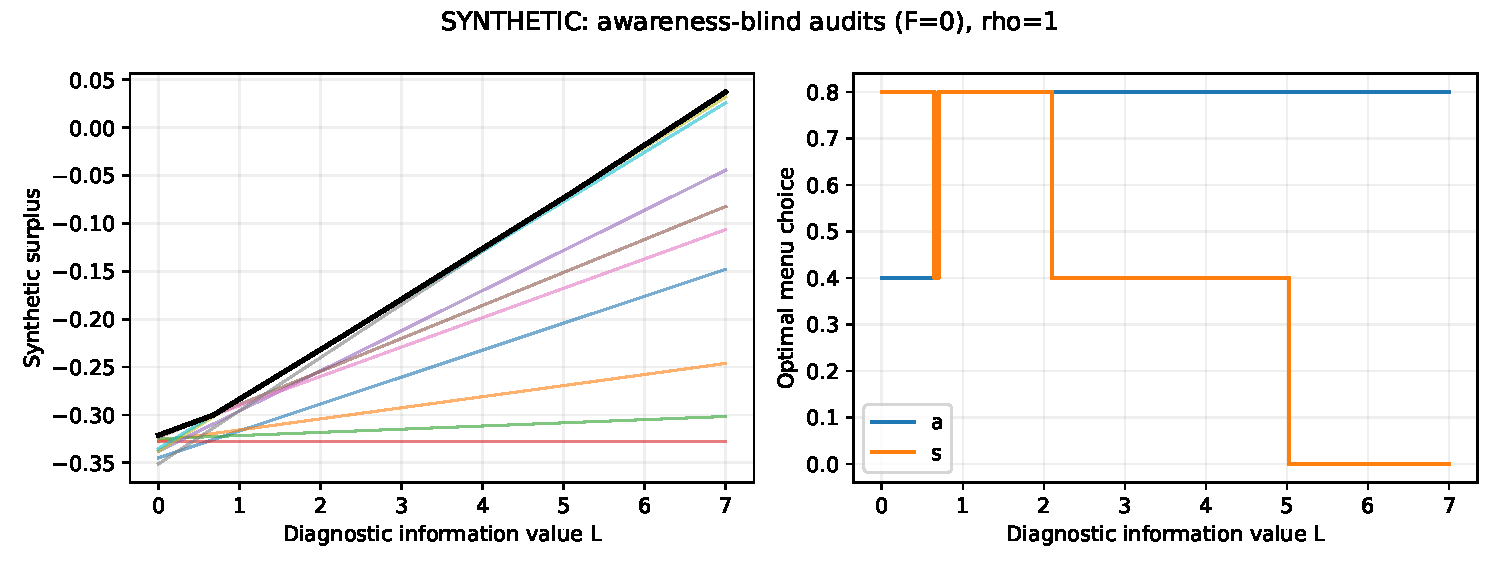
\includegraphics{results/governance.pdf}
\caption{Synthetic global surplus envelope and optimal audit/report-use
choices. All policies have F=0.}
\end{figure}

\subsection{5.4 Interpretation and welfare
limits}\label{interpretation-and-welfare-limits}

The reversal in Theorem 5 requires no accusation of dishonesty from an
audit omission. Known charge \(s\) affects disclosure, independent
occurrence charge \(b\) affects prevention, and a higher audit package
can supply more diagnostic labels. A protected channel is optimal in
some parameter regions and not others. The earlier two-policy comparison
is a special pair of inequalities in (15), not the governance rule.

The finite-menu restriction matters. Additional continuous audit
choices, alternative reporting rewards, leniency schedules, or
outcome-contingent contracts may remove the particular switch or
dominate every menu policy. The theorem is a robust existence result
within an explicit constrained environment, not a universal comparative
static. Its envelope geometry is standard. Its candidate contribution is
the economic nonmonotonicity with separately produced information and
feasible awareness-blind enforcement.

The learning microfoundation is deliberately bounded to one diagnostic
opportunity per independent root cause. Repeated reports about the same
cause would saturate value and must not be added linearly. Since defects
create opportunities to learn, sufficiently large \(L\) may favor
policies with more remaining defects; prevention harm is explicitly
counted through \(D\), but the assumed future remedy value must be
justified in an application. None of the normalized magnitudes is
calibrated.

\section{6. Verification and evidence
status}\label{verification-and-evidence-status}

The analytical solution is global in worker effort under (6), including
\(d=0\), \(c=0\), \(c=1\), and all finite policy boundaries. The policy
solver compares all twelve candidates and applies the exact liability
rule. It computes the optimality intervals rather than searching only a
grid of \(L\) values. It brackets every feasible policy's unique effort
root with rational endpoints and propagates those brackets using
50-digit interval arithmetic. All nonadjacent inequalities needed for
the stated regions are certified; adjacent intersections are enclosed
and strictly ordered. Thus the numerical counterexample is
computer-assisted, with executable interval checks, not inferred from a
graph.

Independent floating-point checks compare direct three-choice
optimization to the analytical response in 126 cases across \(F=0\),
hypothetical \(F=1\), policy boundaries, and concealment corners. Finite
differences agree with (8) to less than \(8\times10^{-12}\) on the
checked interior cases. A separate low-remediation example gives exactly
zero attention. These checks supplement rather than replace the proof.
Package outputs report solver versions and all synthetic inputs.

No real data were used. The measurement appendix distinguishes
policy-specific actual defect incidence, reporting sensitivity, and
false alarms. It preserves imperfect-audit assumptions and explains the
nonidentification of discovery versus concealment without awareness
data. The proposed study, participant scripts, dictionary, precision
planning, and future-result templates are in a separate protocol,
outside the theoretical results. Neither numerical root verification nor
a pre-analysis plan supplies empirical validity.

\section{7. Conclusion}\label{conclusion-and-remaining-objections}

Jointly choosing auditing and report use changes the policy conclusion.
Without enforceable awareness evidence, the direct fixed-incidence
audit-reversal mechanism disappears. Nevertheless, awareness-blind audit
design can produce a nonmonotone optimal demand for protection when
independent diagnostic information substitutes for worker reports. This
is established globally for a constrained menu, with explicit parameter
regions and robust strict-winner certificates.

The strongest remaining scientific objection is scope. The menu and cost
technology are imposed, continuous and richer contracts are not
optimized, and the general investigation-versus-liability tradeoff is
well established. The article adds a bounded nonmonotonicity result and
an implementability correction, not proof of broad priority or
leading-journal suitability. A consequential empirical application would
still require independent source artifacts, validated audit quality,
credible enforcement of report-use restrictions, and sufficient
organizational policy variation. No publication or outside contact has
been undertaken.


{
\small
\setlength{\parindent}{0pt}
\section*{References}\label{references}

Dai, Chifeng. 2026. ``The interplay of regulatory auditing and
self-auditing: crowd in or out?'' \emph{Journal of Regulatory Economics}
69, article 16. Published 11 May 2026.
\url{https://doi.org/10.1007/s11149-026-09514-2}.

Bénabou, Roland, and Jean Tirole. 2016. ``Bonus Culture: Competitive
Pay, Screening, and Multitasking.'' \emph{Journal of Political Economy}
124(2): 305-370. \url{https://doi.org/10.1086/684853}. March 2013 author
manuscript consulted separately:
\url{https://www.princeton.edu/~rbenabou/papers/Multitasking\%20March\%2019\%20paper.pdf}.

Bernstein, Ethan S. 2012. ``The Transparency Paradox: A Role for Privacy
in Organizational Learning and Operational Control.''
\emph{Administrative Science Quarterly} 57(2): 181-216.
\url{https://doi.org/10.1177/0001839212453028}. Primary institutional
record:
\url{https://dash.harvard.edu/entities/publication/73120378-fdcc-6bd4-e053-0100007fdf3b}.

Edmondson, Amy C. 1996. ``Learning from Mistakes is Easier Said Than
Done: Group and Organizational Influences on the Detection and
Correction of Human Error.'' \emph{Journal of Applied Behavioral
Science} 32(1): 5-28. \url{https://doi.org/10.1177/0021886396321001}.

Graff Zivin, Joshua, and Alexander S. P. Pfaff. 2004. ``To err on humans
is not benign: Incentives for adoption of medical error-reporting
systems.'' \emph{Journal of Health Economics} 23(5): 935-949.
\url{https://doi.org/10.1016/j.jhealeco.2004.01.003}. Published
author-hosted article:
\url{https://people.duke.edu/~asp9/files/AuditingMedicalErrorsPublished.pdf}.

Kaplow, Louis, and Steven Shavell. 1994. ``Optimal Law Enforcement with
Self-Reporting of Behavior.'' \emph{Journal of Political Economy}
102(3): 583-606. \url{https://doi.org/10.1086/261947}. Distinct earlier
working version: NBER Working Paper 3822, 1991,
\url{https://doi.org/10.3386/w3822}.

Maas, Victor S., and Marcel van Rinsum. 2013. ``How Control System
Design Influences Performance Misreporting.'' \emph{Journal of
Accounting Research} 51(5): 1159-1186.
\url{https://doi.org/10.1111/1475-679X.12025}.

Pfaff, Alexander S. P., and Chris William Sanchirico. 2000.
``Environmental Self-Auditing: Setting the Proper Incentives for
Discovery and Correction of Environmental Harm.'' \emph{Journal of Law,
Economics, \& Organization} 16(1): 189-208.
\url{https://doi.org/10.1093/jleo/16.1.189}. Primary author record:
\url{https://sites.sanford.duke.edu/alexpfaff/2000/01/09/environmental-self-auditing-setting-the-proper-incentives-for-discovery-and-correction-of-environmental-harm/}.

Strausz, Roland. 2006. ``Buried in paperwork: Excessive reporting in
organizations.'' \emph{Journal of Economic Behavior \& Organization}
60(4): 460-470. \url{https://doi.org/10.1016/j.jebo.2004.10.004}.
Earlier manuscript consulted separately: SFB/TR 15 Discussion Paper 27,
19 October 2004, \url{https://epub.ub.uni-muenchen.de/13521/1/27.pdf}.

Wang, Shouqiang, Francis de Véricourt, and Peng Sun. 2024. ``Audit and
Remediation Strategies in the Presence of Evasion Capabilities.''
\emph{Operations Research} 72(5): 1843-1860. First online 10 July 2024.
\url{https://doi.org/10.1287/opre.2022.0289}. Author manuscript
consulted:
\url{https://personal.utdallas.edu/~sxw163830/papers/Evasion.pdf},
unversioned 57-page file; theorem numbering in the comparison refers to
that manuscript.

}
\clearpage
\section{Appendix A. Complete
proofs}\label{appendix-a.-complete-proofs}

\subsection{A.1 Global response, including inactive
attention}\label{a.1-global-response-including-inactive-attention}

For any discovered defect, the bracketed expression in (2) is strictly
concave in \(c\), with derivative \(s-v-aF-\eta c\). Maximizing on
\([0,1]\) yields (5). For given \(e\), the attention problem is
\(\max_{0\leq d\leq1}\{pdg-kd^2/2\}\). It gives \(d=[pg/k]_0^1\). Under
(6) no positive attention can saturate, so \(d=pg_+/k\), including
\(g\leq0\).

Substituting both choices gives reduced utility

\[\widetilde U(e)=-c_e e^2/2-Hp+p^2g_+^2/(2k).\]

Its first and second derivatives are

\[\widetilde U_e=-c_e e+Hp-p^2g_+^2/k,\]
\[\widetilde U_{ee}=-c_e-Hp+2p^2g_+^2/k.\]

Because \(p\leq p_0\), (6) implies \(H-2pg_+^2/k>0\), so the second
derivative is strictly negative everywhere. At zero effort the first
derivative is \(p_0(H-p_0g_+^2/k)>0\); it tends to minus infinity as
effort grows. Exactly one positive maximum therefore solves (7).
Attention is then unique. Continuation concealment is unique conditional
on a discovery by strict concavity; if \(d=0\) no realized concealment
frequency can be inferred. Strict monotonicity of the effort equation
and its nonzero derivative give continuous dependence on parameters,
including \(g=0\) and concealment corners. Since \(g_+^2\) is
differentiable at \(g=0\) with derivative zero, no discontinuity in
effort appears there. This proves Theorem 1.

\subsection{A.2 Feasible audit derivatives and report-use
decomposition}\label{a.2-feasible-audit-derivatives-and-report-use-decomposition}

With \(F=0\), the continuation optimization (5) has no \(a\) dependence.
This proves fixed-incidence invariance without any interior assumption:
even the truncated attention function is unchanged. Differentiate the
effort equation \(f=c_e e-Hp+p^2g_+^2/k=0\). Its effort derivative is
\(\Delta>0\). Since \(f_a=-pb\), the implicit function theorem gives
\(e_a=pb/\Delta\). Therefore \(p_a=-pe_a\). With \(q=p g_+(1-c)/k\) and
\(g,c\) independent of \(a\), \(q_a=-e_aq\), including \(g_+=0\) and
\(c=1\). This proves (8) and Theorem 2 at every audit boundary by
one-sided differentiation.

Where \(0<c<1\) and \(g>0\), the envelope theorem gives \(g_s=-(1-c)\)
and \(c_s=1/\eta\). Holding \(e\) fixed, \(f_s=2p^2g g_s/k=-2pd(1-c)\);
hence \(e_s=2pd(1-c)/\Delta\). Differentiating \(q=p g(1-c)/k\) yields
(9). For \(c=0\) or \(c=1\), use its zero local derivative; at a
switching boundary use adjacent one-sided derivatives. At \(g=0\), \(q\)
is continuous with the one-sided derivative inherited from the
positive-attention branch. In no case does a report omission identify
its cause.

For (10), a diagnostic label arrives through a report, or through an
audit when no report supplied the label. Conditional independence gives
\(q+a\rho(1-q)\). The same argument with \(\rho=1\) gives occurrence
detection. Substituting (8) and \(p_a=-pe_a\) and differentiating proves
(11). This derivation makes the prevention term explicit rather than
mixing it with the fixed-incidence derivative.

\subsection{A.3 Primitive fixed-incidence reversal and every
boundary}\label{a.3-primitive-fixed-incidence-reversal-and-every-boundary}

Fix \(p\) and \(F>0\). In the interior concealment region
\(c=(x-aF)/\eta\), so \(c_a=-F/\eta\). Substituting the continuation
optimum into \(g\) gives \(g=u-x+\eta c^2/2\) and \(g_a=-Fc\). With
positive unsaturated attention,

\[q=pg(1-c)/k,\] \[q_a=(p/k)[-Fc(1-c)+gF/\eta]
 =(pF/k)[(u-x)/\eta+\tfrac32c^2-c].\]

The quadratic is negative strictly between its distinct real roots. Its
discriminant is \(1-6t\), giving (13). One must also require \(g>0\),
\(0<c<1\), unsaturated attention, and a reachable audit intensity. Those
restrictions are part of the result; roots alone do not establish a
feasible reversal. The minimum of \(\tfrac32c^2-c\) over the real line
is \(-1/6\), at \(c=1/3\). Hence \(t\geq1/6\) rules out a negative
derivative.

If attention is saturated, \(q=1-c\) and \(q_a=F/\eta>0\) in interior
concealment. If \(g<0\), attention and reporting are zero locally. If
\(c=0\) on an open interval, \(g=u-x\) is independent of \(a\) and \(q\)
is constant. If \(c=1\) on an open interval, \(q=0\) regardless of
attention. The truncation maps and continuation value are continuous at
\(g=0\), \(c=0\), \(c=1\), and \(pg=k\), so the one-sided formulas
exhaust their boundaries. When \(F=0\) the continuation problem is
independent of audit intensity for every \(p\), including saturation, so
all fixed-incidence changes vanish. This proves Theorem 3 globally as a
piecewise statement.

\subsection{A.4 Full policy regions and monotonic
information}\label{a.4-full-policy-regions-and-monotonic-information}

The finite feasible set is nonempty in the example and, in general, is
assumed nonempty. It has a global maximizer because it is finite. For
any candidate \(j\), \(W_j\geq W_i\) for every \(i\) is both necessary
and sufficient for global optimality; substitution yields (15).
Expanding one inequality gives the explicit halfspace

\[D(p_i-p_j)+L(I_j-I_i)+M(T_j-T_i)
 -\frac{\kappa}{2}(a_j^2-a_i^2)
 -\gamma[\phi(s_j)-\phi(s_i)]\]
\[\hspace{1cm}+u(p_jd_j-p_id_i)-(E_j-E_i)\geq0. \tag{A1}\]

Conditional on worker primitives, all coefficients are fixed. A pair
with greater \(I_j\) supplies a lower bound on \(L\), one with smaller
\(I_j\) supplies an upper bound, and equal slopes are decided by
intercepts. Intersecting with \(L\geq0\) yields (16), including empty
regions and ties. The menu's endpoints need no separate first-order
conditions; they are compared directly.

Take \(L_2>L_1\) and optimal policies \(j_1,j_2\). Optimality gives

\[B_{j_1}+L_1I_{j_1}\geq B_{j_2}+L_1I_{j_2},\]
\[B_{j_2}+L_2I_{j_2}\geq B_{j_1}+L_2I_{j_1}.\]

Adding yields \((L_2-L_1)(I_{j_2}-I_{j_1})\geq0\). Thus optimal \(I\) is
weakly increasing even with ties. The proof does not order any component
of the policy pair. Equation (17) follows by expanding (10), and solving
its sign inequality under the corollary's assumptions proves (18) and
the pairwise crossing claim. This proves Theorem 4 and Corollary 4.1.

\subsection{A.5 Certificate and robustness proof for Theorem
5}\label{a.5-certificate-and-robustness-proof-for-theorem-5}

All decimal primitives in Section 5.3 are exact rational numbers. The
unique effort for each feasible policy is the root of a strictly
increasing \(f(e)\), with \(f(0)<0<f(8)\). The reproduction script
performs rational bisection and evaluates the sign of \(f\) using
outward interval arithmetic. Each nonambiguous sign discards the
corresponding half interval without excluding the root. After 120 steps
the rational bracket encloses the unique root; propagating its endpoints
through \(p,d,q,E,B,I\) produces interval coefficients. No
floating-point point estimate is used as a proof of a sign.

For adjacent policies \(j_m,j_{m+1}\) in the displayed sequence, the
exact threshold is

\[t_m=(B_{j_m}-B_{j_{m+1}})/(I_{j_{m+1}}-I_{j_m}).\]

The interval coefficients enclose these roots as reported, with strictly
positive denominators and strictly ordered thresholds. For each active
policy the script checks every nonadjacent inequality in (16): each
competing lower threshold lies strictly below its left active endpoint
and each competing upper threshold strictly above its right active
endpoint. Adjacent inequalities hold by the definition of \(t_m\).
Equal-policy comparisons are identities. This certifies the claimed
intervals against all feasible policies for every \(L\geq0\), including
both unbounded outer regions. At each endpoint only the adjacent
policies tie because all nonadjacent comparisons are strict.

As a second certificate, at \(L=0,.66,1,3,6\), respectively, the minimum
surplus margin over every other feasible policy at \(\rho=1\) exceeds \$
.0023867,.0001148,.0013744,.0011285,.0026163\$. The script also
certifies strict positivity at \(\rho=.8\) for each same witness and
every competitor. Differences at a fixed witness are affine in \(\rho\),
so endpoint positivity proves positivity on the entire interval
\([.8,1]\). Hence the five optimal choices, including the increase of
\(s\) from \(.4\) at \(.66\) to \(.8\) at \(1\), persist for each such
audit quality. Worker responses and surplus coefficients are continuous
in all the remaining continuous primitives by Theorem 1. Strict finite
sets of witness inequalities therefore persist on an open neighborhood;
choose an interior \(\rho\), such as \(.9\), for a full
relative-interior robustness statement.

The cap \(B=2.8\) places a candidate on its liability boundary. For
robustness take caps in \((2.8,3.2)\), which preserve the same feasible
set: \(s=.8\) remains feasible at positive \(a\), \(s=1.2\) remains
infeasible. Thus there is an ordinary open cap interval as well, rather
than incorrectly claiming a two-sided neighborhood around a feasibility
discontinuity. For \(B=2.4\) the finite set changes, and direct
all-policy comparison at \(L=0\) gives the stated different optimum.
These arguments prove Theorem 5 as a computer-assisted existence and
parameter-region result.

\subsection{A.6 Accountability can also reward
documentation}\label{a.6-accountability-can-also-reward-documentation}

The corruption baseline is not a universal prediction. Suppose
accountability additionally increases the real private benefit of
investigation, \(u(s)=u_0+\omega s\), and independently verified effort
incentives enter as \(H(s)=h+ab+\chi s\). In an interior concealment
region, \(g_s=\omega-(1-c)\) and the same differentiation gives

\[e_s=[p\chi-2pdg_s]/\Delta,\] \[q_s=-e_sq+pg_s(1-c)/k-d/\eta.\]

Thus genuine prevention and sensitivity can rise together if
\(\chi>2dg_s\) and \(pg_s(1-c)/k>e_sq+d/\eta\). These conditions follow
directly from the derivatives and are not field estimates. At
concealment corners omit the \(d/\eta\) term locally. This alternative
changes worker primitives and therefore requires recomputing every
policy region; it is not silently built into the certified baseline.

\section{Appendix B. Measurement and limits of
identification}\label{appendix-b.-measurement-and-limits-of-identification}

The operational unit is a completed item and policy can be assigned by
team. Define \(p_t=\Pr(Z(t)=1)\), \(q_t=\Pr(R(t)=1\mid Z(t)=1)\), and
\(f_t=\Pr(R(t)=1\mid Z(t)=0)\). They satisfy

\[\Pr(R(t)=1)=p_tq_t+(1-p_t)f_t.\]

A report count alone does not separate these quantities. Moreover,
\(q_t\) concerns each policy's own defect population. A contrast in
\(q_t\) is not a behavioral effect among the latent items defective
under both policies. Severity-standardized comparisons are secondary and
do not identify that principal stratum.

Let audit selection have known positive inclusion probability \(\pi_i\).
Probability weighting identifies the joint table of auditor
classification \(Y\) and recording \(R\) under complete follow-up or an
explicitly justified missingness model. Let validated audit sensitivity
and specificity be \(\alpha,\beta\), and assume \(Y\perp R\mid Z,t,X\).
For each report status \(j\),

\[\begin{pmatrix}P(Y=0,R=j)\\P(Y=1,R=j)\end{pmatrix}
=\begin{pmatrix}\beta&1-\alpha\\1-\beta&\alpha\end{pmatrix}
\begin{pmatrix}P(Z=0,R=j)\\P(Z=1,R=j)\end{pmatrix}. \tag{B1}\]

The matrix determinant is \(\alpha+\beta-1\). If this is nonzero and the
error rates are known, inversion identifies the latent joint table;
summing its true-defect row gives \(p\), dividing its \((Z=1,R=1)\) cell
by \(p\) gives \(q\), and dividing its \((Z=0,R=1)\) cell by \(1-p\)
gives \(f\). Sensitivity is undefined at \(p=0\), false alarms at
\(p=1\). The usual informative-audit restriction is \(\alpha+\beta>1\).
If error rates vary by report status, treatment, or covariate stratum,
each required matrix must be validated separately.

This is standard misclassification algebra, not a new estimator.
Negative inverse cells in samples are a warning, not an invitation to
truncate silently. Use a constrained likelihood and propagate validation
uncertainty. Bounds over feasible latent tables and validated error
ranges replace point estimates when accuracy is uncertain. Two reviewers
of the same incomplete source do not automatically create a gold
standard. Missing audits and nonrandom selection require explicit
adjustment assumptions or bounds. Organizational auditing capability
\(\rho\) is not estimated by merely counting research-audit
disagreements: diagnostic labels need their own validation.

Without observed awareness, \(q=d(1-c)\) does not identify its
components. For any \(q\in(0,1)\), \((d,c)=(q,0)\) and \((1,1-q)\) both
reproduce it. Occurrence audits, even perfect ones, cannot discriminate
these behaviors without additional information or exclusion
restrictions. A timestamped draft can establish awareness in a subset
but does not exhaust all awareness; conditioning on drafts selects a
post-treatment subset. This nonidentification remains even though the
theoretical worker model has separate choices. The empirical protocol
must therefore estimate policy-specific reporting sensitivity, not claim
a causal decomposition into discovery and dishonesty.

\end{document}
